% Book pp. 79-81 (PDF pp. 80-82)
\section{Solving Systems of Quadratic Inequalities}

We have explored how to solve single quadratic inequalities algebraically and
graphically. Now, we will learn how to solve systems of quadratic inequalities
(two or more quadratic inequalities) through algebra and graphing.

In finding solutions to quadratic inequalities algebraically, you solve them
simultaneously.

\begin{example}{Example 2.20}
Graph the system of quadratic inequalities $y \ge 4x^2 + 5x$, $y < -3x^2 - 7x$.

\solution
\textit{Solving the systems of inequalities simultaneously}

\textbf{Step 1:} Equate the two expressions

$4x^2 + 5x = -3x^2 - 7x$

\textbf{Step 2:} Simplify and make $x$ the subject.
\begin{align*}
  4x^2 + 3x^2 + 7x + 5x &= 0 \\
  7x^2 + 12x &= 0 \\
  x(7x + 12) &= 0 \\
  x = 0,\ x &= -\frac{12}{7}.
\end{align*}
\textbf{Step 3:} Identify whether the point of intersection is inclusive in the solution to
the systems.

Since the $y < -3x^2 - 7x$ has the strictly $<$ symbol, the points of intersection will
not satisfy this inequality.

For $y \ge 4x^2 + 5x$,

At $x = 0$, $y \ge 4(0)^2 + 5(0)$,

$y \ge 0$.

For $y < -3x^2 - 7x$,

At $x = 0$, $y < -3(0)^2 - 7(0)$,

$y < 0$

At $x = 0$, y must be 0 in both inequalities, but since the second inequality requires
$y < 0$, there is no solution at this point.

At $x = \frac{-12}{7}$, $y \ge 4\left(\frac{-12}{7}\right)^2 + 5\left(\frac{-12}{7}\right)$,

$y \ge 3\frac{3}{49}$.

At $x = 0$, $y < -3\left(\frac{-12}{7}\right)^2 - 7\left(\frac{-12}{7}\right)$,

$y < \frac{156}{49}$.

$y < 3\frac{9}{49}$.

At $x = \frac{-12}{7}$, y must be $3\frac{9}{49}$ in both inequalities, but since the second
inequality requires $y < 3\frac{9}{49}$, there is no solution at this point.
\booknote{$4\left(\frac{-12}{7}\right)^2 + 5\left(\frac{-12}{7}\right) = \frac{156}{49}
= 3\frac{9}{49}$, so ``$y \ge 3\frac{3}{49}$'' is a misprint; the line ``At $x = 0$,
$y < -3\left(\frac{-12}{7}\right)^2 \ldots$'' should begin ``At $x = \frac{-12}{7}$''.}

\textbf{Step 4:} State the solution

Since the points of intersection will not satisfy one of the inequalities, the solution
becomes $-1\frac{5}{7} < x < 0$. That is, the region between the points of intersection.

\medskip\noindent{\large\textbf{Solving the systems of inequalities graphically}}

\textbf{Step 1:} Draw the graphs of the two inequalities.
\begin{center}
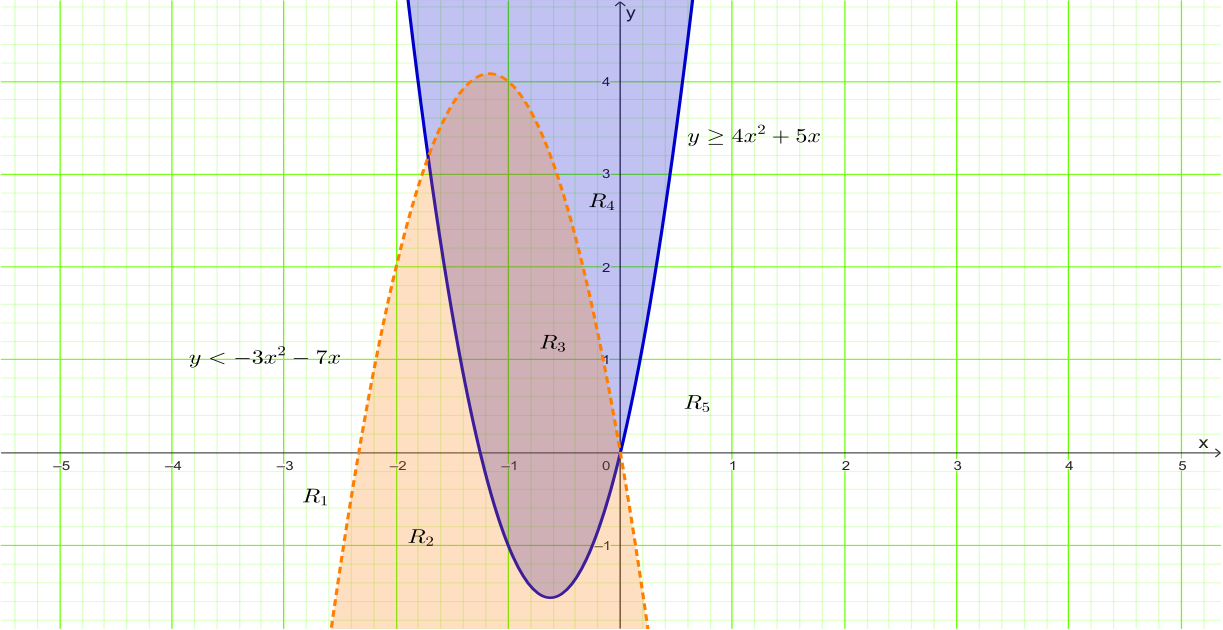
\includegraphics[width=0.9\linewidth]{figures/fig2-11.png}
\end{center}
\figcaption{2.11}{Graphical Solution to $y \ge 4x^2 + 5x$, $y < -3x^2 - 7x$}

\textbf{Step 2:} Identify the region that is common to both inequalities.

$R_3$

\textbf{Step 3:} State the solution to the system of inequalities.

$-1\frac{5}{7} < x < 0$

\textbf{Step 3:} State the conclusion.

All points in the region $R_3$ including but not exclusive to $(-1, 0)$, $(-1, 3)$
$(-0.5, 2)$, $(-1, 1)$ and $(-0.5, -1)$ are in the solution set for the system.
\end{example}

\begin{example}{Self-assessment task}
Find the solution to $y < -7x^2 - 8x + 3$ and $y > 3x^2 - 7x$.

You should find $-0.6 < x < 0.5$
\end{example}
